\documentclass[conference]{IEEEtran}
\usepackage{cite,amsmath,amssymb,graphicx,booktabs,array,url,textcomp}
\hyphenation{XGBoost}
\begin{document}
\title{Predicting a Water Quality Index Without Data Leakage: Gradient Boosting Compared with a Deep Neural Network}
\author{\IEEEauthorblockN{T109: Priyal, Anusha, Sarthak, Kashika and Vaishnavi}
\IEEEauthorblockA{Newton School of Technology\\
Advanced Machine Learning / Deep Learning, Project 18 (Phase 2)\\
Code: \url{https://github.com/Priyal-2005/water-quality-prediction}}}
\maketitle
\begin{abstract}
A water quality index turns several measurements into one score between 0 and 100. In Phase 1 we predicted the CCME index from a small set of readings, hiding the five measurements that the index is mostly built from, and found that XGBoost was the best of four classical models. In Phase 2 we train a small neural network (a multilayer perceptron, MLP) on the same inputs, splits and metrics, and compare it with XGBoost on monitoring stations neither model has seen. On the test stations the MLP (RMSE 11.108, R$^2$ = 0.287) and XGBoost (RMSE 11.058, R$^2$ = 0.293) cannot be told apart: the paired 95\% interval for the RMSE difference is $-$0.053 to $+$0.147. On later years the MLP is slightly better (RMSE 7.866 against 8.061). A weighted blend of the two models, with its weight chosen on validation data only, gives a small but consistent gain on unseen stations (RMSE 11.010; difference to XGBoost $-$0.049, interval $-$0.098 to $-$0.002). All three models over-predict the quality of polluted water by about 29 points. A leakage check shows why: giving the models the five hidden chemicals lifts validation R$^2$ from about 0.35 to 0.99.
\end{abstract}
\begin{IEEEkeywords}
water quality index, multilayer perceptron, XGBoost, tabular deep learning, data leakage, ensemble
\end{IEEEkeywords}

\section{Introduction}
A water quality index combines many measurements into one number that is easy to report and compare. A model that predicts this number from a few simple readings could help with screening, but only if the test is fair: if the model is given the measurements the index is calculated from, it can just recompute the formula.

In Phase 1 we predicted \texttt{target\_ccme\_value}, the CCME index (0 to 100, higher is cleaner), from 14 inputs and compared a baseline, Ridge Regression, Random Forest and XGBoost. XGBoost was best, with test R$^2$ = 0.293 on unseen stations. In Phase 2 we ask whether a neural network can do better on the same task. Published studies on tabular data suggest that it often cannot~\cite{grinsztajn2022,shwartz2022,borisov2022,mcelfresh2023}, so we treat the question as a fair test and not as a race. Our contributions are:
\begin{itemize}
\item an MLP trained and tuned on the validation data only, scored once on the test data;
\item a paired comparison with XGBoost using the same re-drawn stations, so that the difference between models has its own confidence interval;
\item a simple weighted blend of the two models (optional hybrid), and a check of a more complex residual-learning version that we rejected;
\item an experiment showing what happens if the five hidden chemicals are given to the models.
\end{itemize}
The code, data and results are in our GitHub repository: \url{https://github.com/Priyal-2005/water-quality-prediction}. Data cleaning, the target and the Phase 1 models are described in our Phase 1 report; we repeat only what is needed here.

\section{Related work}
The CCME index is based on how many measurements break their guideline, how often, and by how much~\cite{ccme2001}. Reviews describe the weaknesses of water quality indices~\cite{chidiac2023}. We use a cleaned part of the dataset of Karim et al.~\cite{karim2025}.

A multilayer network can in principle approximate a very wide class of functions~\cite{hornik1989} and is trained by back-propagation~\cite{rumelhart1986}; we use the Adam optimiser~\cite{kingma2015}. Dropout~\cite{srivastava2014} and early stopping~\cite{prechelt1998} reduce overfitting. For tables of mixed numbers and categories, several studies found that tree models such as XGBoost~\cite{chen2016} are still as good as or better than deep models~\cite{grinsztajn2022,shwartz2022,borisov2022}. Gorishniy et al.\ found that neither family is better everywhere~\cite{gorishniy2021}, and McElfresh et al.\ found the gap often negligible, with light tuning of a tree model mattering more than the choice of family~\cite{mcelfresh2023}. Shwartz-Ziv and Armon also found that an ensemble of deep models and XGBoost did better than XGBoost alone~\cite{shwartz2022}; the idea of combining two forecasts goes back to Bates and Granger~\cite{bates1969}.

Deep learning has been used for water quality and hydrology~\cite{sit2020}. Zhi et al.\ trained an LSTM on dissolved oxygen in 236 US watersheds and found it useful in basins without measurements but weaker at peaks and troughs~\cite{zhi2021}. Rahman et al.\ reported 97.33\% accuracy for five CCME classes on the Canadian part of the dataset we use, with the eight index measurements as inputs~\cite{rahman2026}. Because the index is calculated from those eight, such scores cannot be compared with ours (Section~\ref{sec:leak}). Our gap is a fair, like-for-like comparison of a neural network and gradient boosting, with uncertainty on the difference between them.

\section{Data and setup}
After cleaning, the dataset has 259,774 rows from 9,940 monitoring stations in England, Ireland, the USA and Canada, from 2000 to 2023; 43.7\% of the targets are exactly 100. The main split is \emph{by station}: all rows of a station go to one part only (181,747 training, 26,054 validation and 51,973 test rows from 6,583, 1,136 and 2,221 stations). The second split is \emph{by year}: training up to 2015, validation 2016--2017, test 2018 onwards. The index is calculated from eight measurements; we hide ammonia, BOD, orthophosphate, nitrogen and nitrate and keep 14 inputs: dissolved oxygen, pH, temperature, month (sine and cosine), oxygen saturation, dissolved oxygen $\times$ temperature, the station's average past dissolved oxygen, pH and temperature (earlier dates only), the number of earlier samples, days since the previous sample, water body type and country. Missing values are filled with training medians and flagged. After one-hot coding and the flags the network receives 30 columns. The random seed is 42 everywhere, and the test set is scored once, after all choices are made.

\section{Models and methods}
\subsection{The MLP}
The network has 30 inputs, a hidden layer of 128 units, a hidden layer of 64 units and one output: Linear(30,128), ReLU, Dropout(0.2), Linear(128,64), ReLU, Dropout(0.2), Linear(64,1). It has 12,289 weights for about 182,000 training rows. The output has no activation, because a sigmoid would flatten the many scores near 100. The target is standardised with training statistics during training and converted back afterwards. The loss is mean squared error, the optimiser is Adam (learning rate 0.001, batch size 512), weight decay is $10^{-4}$, and training stops when the validation loss has not improved for 10 epochs. The weights from the best epoch are kept.

\subsection{Tuning}
We tried 13 settings: our default plus 12 random ones, changing layer sizes, dropout, weight decay, learning rate, loss (MSE or Huber) and batch size. The setting with the lowest validation RMSE was chosen; the test set was never used. The default won. Twelve of the 13 trials landed between validation RMSE 11.23 and 11.41 and the worst was 11.59 (Fig.~\ref{fig:tune}), so the network is not very sensitive to these choices. A Huber loss lowered MAE but raised RMSE, so we kept MSE. Thirteen trials is a small search, so we have not shown that tuning can never help.

\begin{figure}[!t]\centering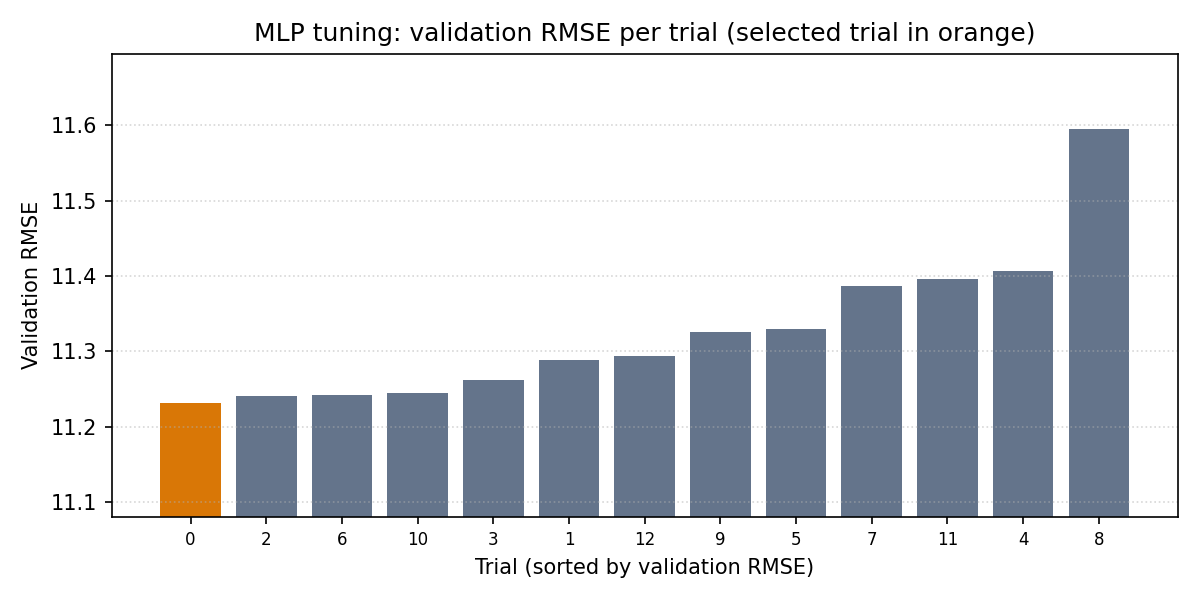
\includegraphics[width=\columnwidth]{../results/dl/figures/mlp_tuning_trials.png}\caption{Validation RMSE of the 13 tuning trials. The default setting was best.}\label{fig:tune}\end{figure}

\subsection{Regularisation}
Training error keeps falling while the validation error stops improving around epoch 19 (Fig.~\ref{fig:curve}); training stopped at epoch 29 and the epoch-19 weights were kept. Tested one at a time, dropout and weight decay changed the validation result very little (Section~\ref{sec:abl}), so they act as cheap safeguards, and early stopping is the part that matters.

\begin{figure}[!t]\centering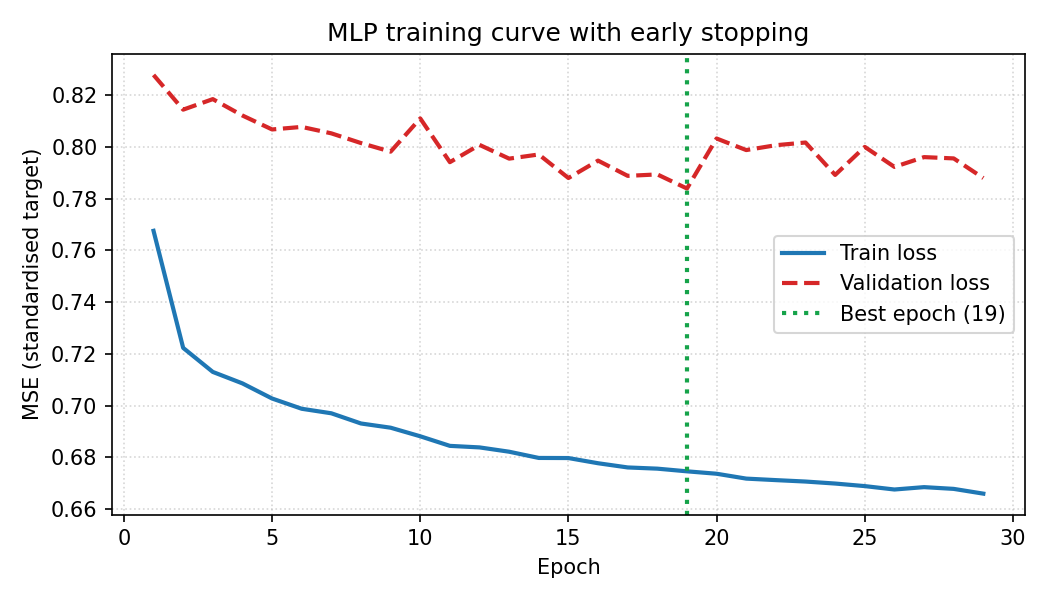
\includegraphics[width=\columnwidth]{../results/dl/figures/mlp_training_curve.png}\caption{Training and validation loss per epoch. Validation stops improving near epoch 19.}\label{fig:curve}\end{figure}

\subsection{Hybrid}
The hybrid is a weighted average of the saved Phase 1 XGBoost predictions and the MLP predictions, clipped to 0--100. The weight is chosen on the validation data only: 55\% XGBoost and 45\% MLP (validation RMSE 11.146; Fig.~\ref{fig:blend}). On the year split we use 50/50. We also tried a residual version, in which a second model learns the first model's errors from out-of-fold predictions. The correlation between the out-of-fold predictions and the true errors was only 0.088 on the station split and $-$0.001 on the year split, so the second model had almost nothing to learn and we rejected it.

\begin{figure}[!t]\centering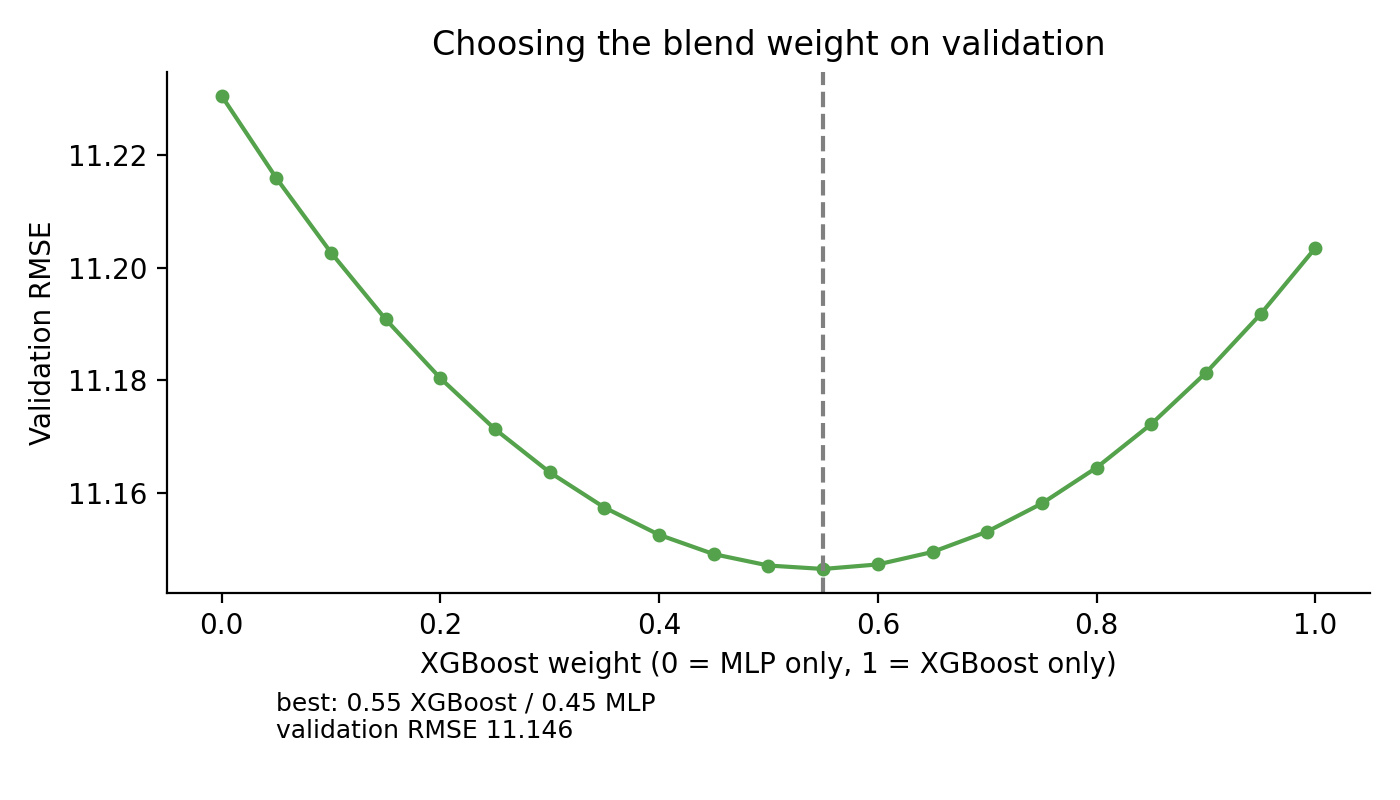
\includegraphics[width=\columnwidth]{../results/dl/figures/hybrid_blend_weight_curve.png}\caption{Validation RMSE for blend weights between the MLP (left) and XGBoost (right).}\label{fig:blend}\end{figure}

\subsection{Metrics and paired intervals}
We report MAE, RMSE and R$^2$ (lower is better for the first two). To show how uncertain a test score is, we re-drew whole stations 2,000 times (seed 42), which keeps the rows of a station together~\cite{efron1979}. The same re-drawn stations are used for every model, so the difference in RMSE between two models has its own interval; if it excludes zero, the difference is consistent.

\section{Results}
\subsection{Validation}
On the validation stations XGBoost has RMSE 11.205 (R$^2$ = 0.348), the MLP 11.231 (0.345) and the hybrid 11.146 (0.355). Random Forest, from Phase 1, is 11.247. The gaps are about 0.03, too small to rank the models on validation alone.

\subsection{Test on unseen stations}
\begin{table}[!t]\caption{Test results on unseen stations (95\% bootstrap intervals for R$^2$).}\centering
{\footnotesize\setlength{\tabcolsep}{3pt}\begin{tabular}{>{\raggedright\arraybackslash}p{0.30\linewidth}rrrr}\toprule
\textbf{Model} & \textbf{MAE} & \textbf{RMSE} & \textbf{R$^2$} & \textbf{95\% CI for R$^2$}\\\midrule
XGBoost & 7.543 & 11.058 & 0.293 & [0.244, 0.341]\\
MLP & 7.606 & 11.108 & 0.287 & [0.236, 0.336]\\
\textbf{Hybrid} & \textbf{7.521} & \textbf{11.010} & \textbf{0.300} & [0.249, 0.347]\\
\bottomrule\end{tabular}}
\end{table}

\begin{table}[!t]\caption{Paired RMSE differences on the same re-drawn test stations.}\centering
{\footnotesize\setlength{\tabcolsep}{3pt}\begin{tabular}{>{\raggedright\arraybackslash}p{0.42\linewidth}rrr}\toprule
\textbf{Comparison} & \textbf{Mean} & \textbf{95\% interval} & \textbf{Excl.\ 0?}\\\midrule
MLP $-$ XGBoost & $+$0.049 & [$-$0.053, 0.147] & no\\
Hybrid $-$ XGBoost & $-$0.049 & [$-$0.098, $-$0.002] & yes\\
Hybrid $-$ MLP & $-$0.098 & [$-$0.150, $-$0.043] & yes\\
\bottomrule\end{tabular}}
\end{table}

The MLP and XGBoost cannot be separated on unseen stations: the difference in RMSE is $+$0.049 and its interval includes zero. The hybrid is better than both, by 0.049 against XGBoost and 0.098 against the MLP, and both intervals exclude zero, but the gains are small (under 0.5\% of the RMSE of XGBoost) and the upper end of the XGBoost interval is close to zero. Fig.~\ref{fig:test} shows the test RMSE and the paired differences. R$^2$ stays below 0.30 for every model, so most of the variation in the score is not explained.

\begin{figure}[!t]\centering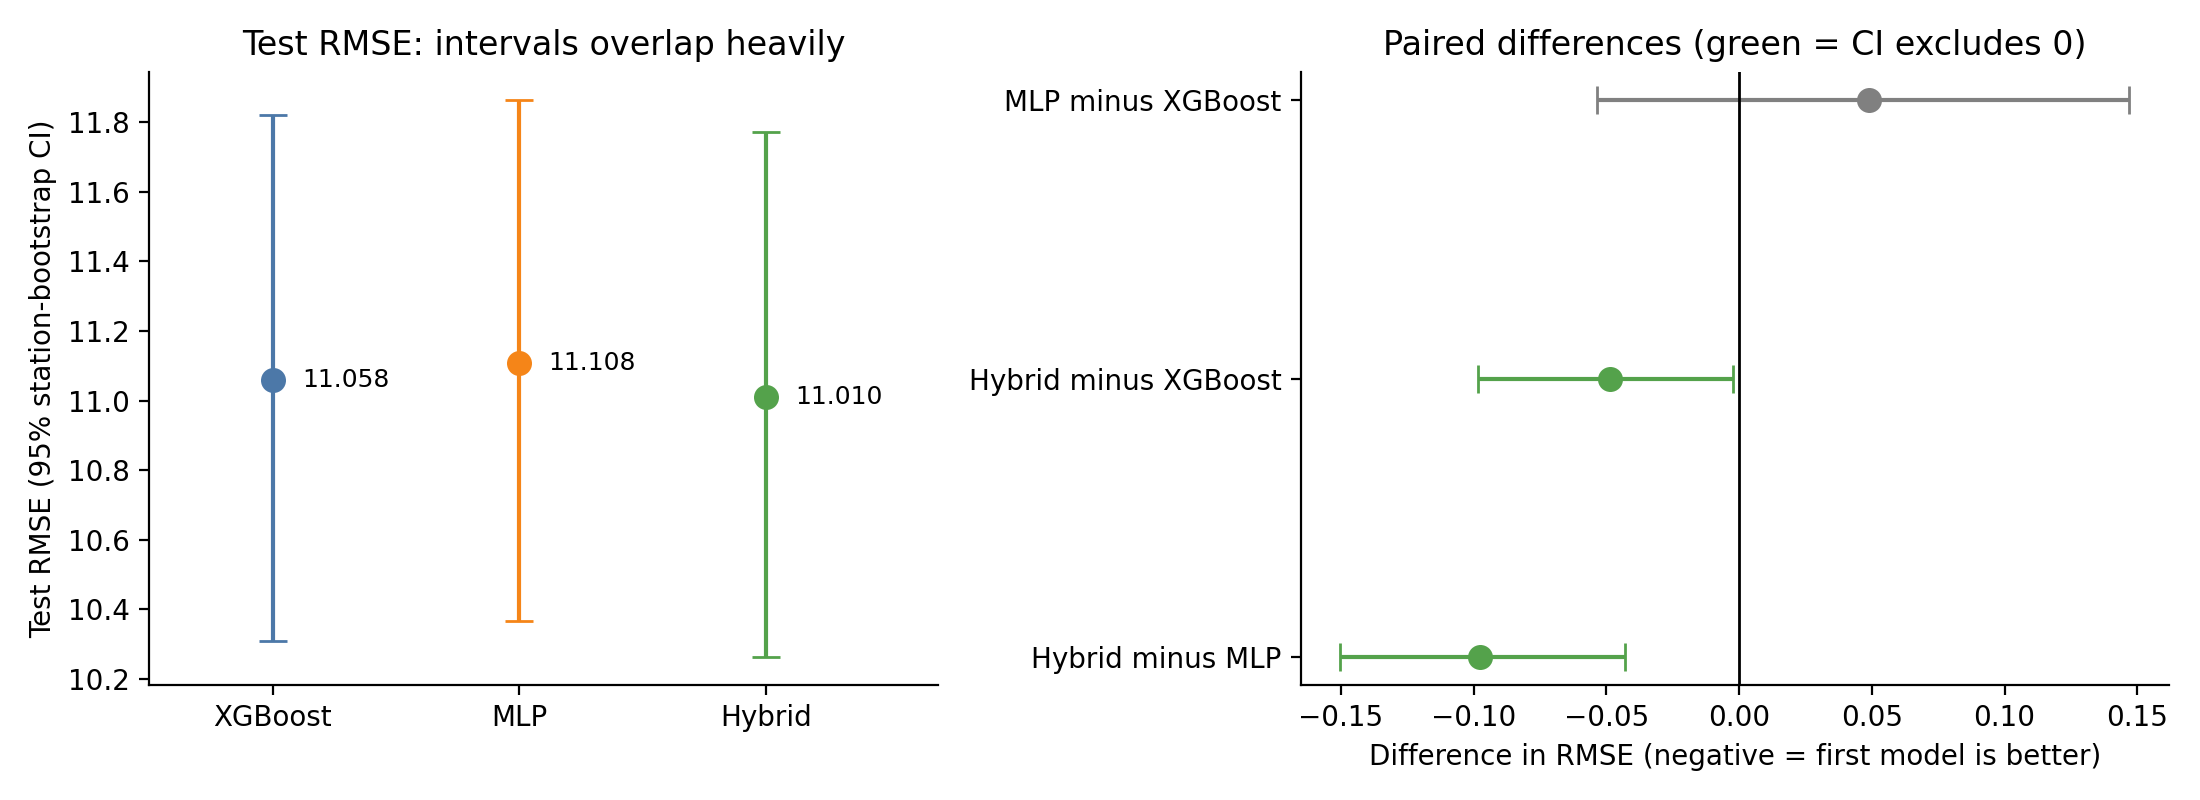
\includegraphics[width=\columnwidth]{../results/dl/figures/station_test_rmse_and_paired_differences.png}\caption{Test RMSE with bootstrap intervals (left) and paired RMSE differences (right).}\label{fig:test}\end{figure}

\subsection{Test on later years}
\begin{table}[!t]\caption{Test results on later years (year split, 2018 onwards).}\centering
{\footnotesize\setlength{\tabcolsep}{3pt}\begin{tabular}{>{\raggedright\arraybackslash}p{0.34\linewidth}rrr}\toprule
\textbf{Model} & \textbf{MAE} & \textbf{RMSE} & \textbf{R$^2$}\\\midrule
XGBoost & 5.469 & 8.061 & 0.240\\
MLP & 5.277 & 7.866 & 0.276\\
\textbf{Hybrid (50/50)} & 5.301 & \textbf{7.842} & \textbf{0.281}\\
\bottomrule\end{tabular}}
\end{table}

On later years the order changes: the MLP is better than XGBoost (RMSE 7.866 against 8.061), and the hybrid is best on RMSE (7.842). We did not compute intervals for this split, so we do not claim that the MLP's lead is significant. These numbers should not be mixed with the station test, because the test data are different. The XGBoost values differ slightly from our Phase 1 report (RMSE 8.047) because the model was retrained inside the Phase 2 evaluation; we use the Phase 2 run so that all three models were scored in the same pipeline.

\subsection{Where do the models go wrong?}
The error analysis below uses the validation stations. All models do well on Excellent and Good water and badly on poor water: the mean error of XGBoost is $-$5.8 points for Excellent water (guesses too low), but $+$25.3 for Marginal and $+$35.7 for Poor water (guesses too high). For water with a true score below 60 (1,755 validation rows) all three models over-predict in almost every row (XGBoost 100\%, MLP 99.9\%, hybrid 100\%) with a mean error of 29.1, 28.9 and 29.0 points. On the year split the same pattern appears (766 rows below 60; mean error 27.9, 29.8 and 28.9). The five chemicals that would show pollution are hidden, so the models cannot tell when water is really bad, and 44\% of samples are exactly 100, so a ``fairly good'' guess is usually safe. Combining models does not fix this, because both models make the same mistake (Fig.~\ref{fig:poll}).

\begin{figure}[!t]\centering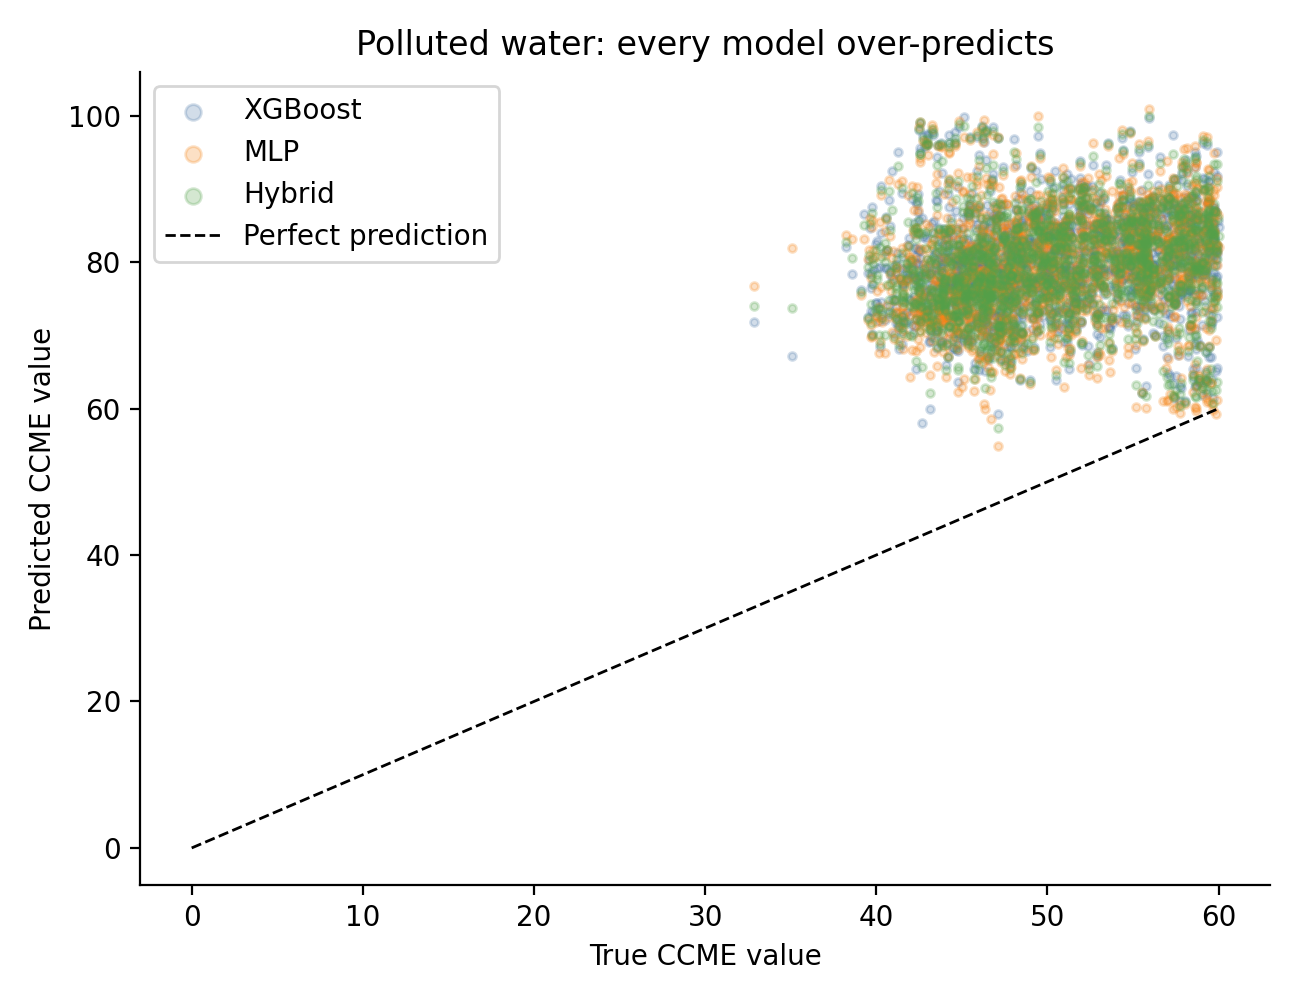
\includegraphics[width=\columnwidth]{../results/dl/figures/polluted_water_pred_vs_actual.png}\caption{Predicted against true score for polluted water: all models over-predict.}\label{fig:poll}\end{figure}

By country (validation), England is the hardest (MAE 9.18 for XGBoost, 9.21 for the MLP, 9.13 for the hybrid), Ireland much easier (3.37, 3.45, 3.37) because 82\% of its samples are exactly 100. The USA (358 rows) and Canada (314 rows) are too small for firm conclusions. On the year split the MLP does better than XGBoost in Ireland (MAE 2.95 against 3.42) and the USA, which is where its overall advantage there comes from.

\subsection{Which design choices matter?}\label{sec:abl}
We changed one setting of the MLP at a time and scored it on the validation stations (Table~\ref{tab:abl}). Depth, width, dropout and weight decay made no clear difference: validation RMSE stayed between 11.23 and 11.37 and the intervals overlap. Removing information mattered most: without the station history RMSE rose to 11.878 and without country to 11.733. So, as in Phase 1, much of the score comes from knowing the country and the station's past, which may not carry over to a new region.

\begin{table}[!t]\caption{One-factor-at-a-time ablations of the MLP (validation RMSE).}\label{tab:abl}\centering
{\footnotesize\setlength{\tabcolsep}{3pt}\begin{tabular}{>{\raggedright\arraybackslash}p{0.55\linewidth}r}\toprule
\textbf{Setting} & \textbf{Val RMSE}\\\midrule
Tuned MLP (128-64, dropout 0.2, wd $10^{-4}$) & 11.231\\
1 hidden layer / 3 hidden layers & 11.369 / 11.279\\
Half width / double width & 11.284 / 11.273\\
No dropout & 11.245\\
No weight decay & 11.245\\
Without station history & 11.878\\
Without country & 11.733\\
\bottomrule\end{tabular}}
\end{table}

\subsection{Leakage check: the five hidden chemicals}\label{sec:leak}
Following examiner feedback we tested what happens if the models may use the five chemicals (ammonia, BOD, orthophosphate, nitrogen and nitrate), on the validation data only (Fig.~\ref{fig:leak}). With our 14 inputs the validation R$^2$ is 0.349 for XGBoost and 0.346 for the MLP. With the five chemicals only it is 0.985 and 0.981, and with both sets 0.991 and 0.986. Both families reach almost the same near-perfect score, so a very high score here shows that the model has re-learned the index formula, not that it predicts water quality from cheap sensors. This is also why accuracy figures built on the index measurements~\cite{rahman2026} are not comparable with ours. The five chemicals are laboratory tests that are expensive and slow, while dissolved oxygen, pH and temperature can come from a cheap sensor; we hide the chemicals on purpose, to keep the prediction task useful and honest.

\begin{figure}[!t]\centering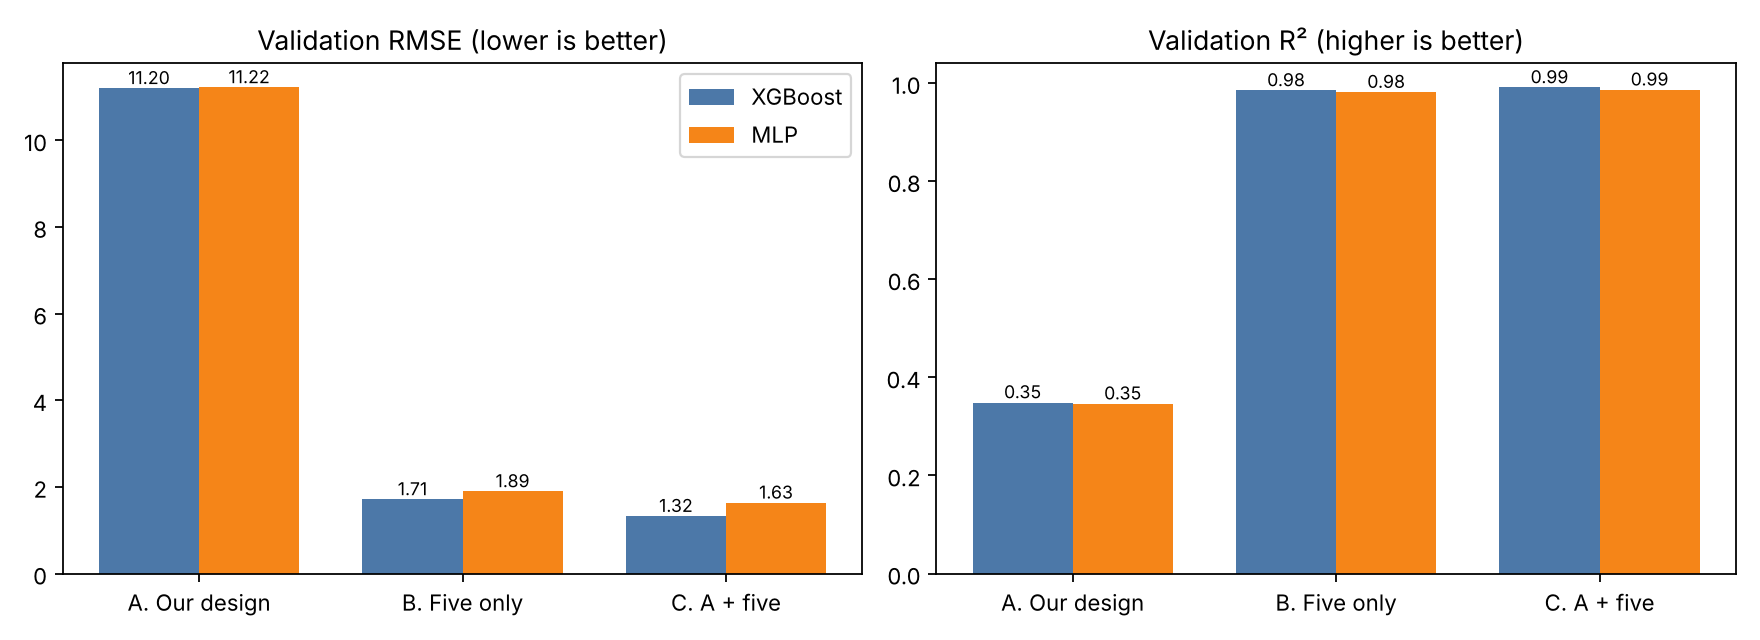
\includegraphics[width=\columnwidth]{../results/dl/figures/five_driver_leakage_check.png}\caption{Validation R$^2$ with our inputs, with the five chemicals only, and with both.}\label{fig:leak}\end{figure}

\section{Discussion}
The literature predicted this result: on a small table of mixed inputs, a plain MLP lands close to a tuned XGBoost and neither family wins everywhere~\cite{gorishniy2021,mcelfresh2023}. The network is slightly worse on unseen stations and slightly better on later years, but only the first comparison has an interval, and it includes zero. The weighted blend helps a little, in line with the older idea of combining forecasts~\cite{bates1969,shwartz2022}. The gain is small because the two models make the same mistakes, and the failed residual experiment shows the same thing from another side. The tuning, the ablations and the leakage check all point one way: the limit is the information in the 14 inputs, not the type of model.

\section{Limitations and future work}
We tried one network design and 13 tuning settings, so a larger search or another architecture could behave differently. We tuned on one validation split without cross-validation, and the test R$^2$ (0.287 for the MLP) is below the validation value (0.345), partly because we chose settings on validation and perhaps because the test stations are harder; we did not separate these reasons. The year split has no confidence intervals. The country and quality-level analyses use the validation stations, and the USA and Canada have few rows. The model cannot replace laboratory tests, and every model is biased towards good scores for polluted water, which is the more harmful mistake. The source data also contain filled-in values that may affect the index. Future work could add inputs that carry information about pollution, such as nearby land use or discharge sites, or train on more stations from the USA and Canada.

\section{Conclusion}
We compared XGBoost, an MLP and a weighted hybrid for predicting the CCME index without the measurements it is calculated from. On unseen stations XGBoost and the MLP are statistically indistinguishable (RMSE 11.058 and 11.108, R$^2$ 0.293 and 0.287); on later years the MLP is slightly better (RMSE 7.866 against 8.061). The 55/45 blend gives the best station score (RMSE 11.010, R$^2$ = 0.300), a small but consistent gain. All models over-predict polluted water by about 29 points, and giving them the five hidden chemicals raises validation R$^2$ from 0.35 to 0.99, which confirms that the index formula, not the model type, decides how high the score can go.

\bibliographystyle{IEEEtran}\bibliography{references_phase2}
\end{document}
